\chapter{El ADN: una molécula genética universal}\label{ch:g10:universal-dna}

En un laboratorio a oscuras, bajo una lámpara azul, uno de dos ratones
blancos brilla en verde del hocico a la cola. Lleva, en cada una de sus
\omterm{def:g10:cells-common-unit:cell}{células}, un solo \omterm{def:g10:universal-dna:gene}{gen} tomado de una medusa que se ilumina en el Pacífico
--- y las \omterm{def:g10:cells-common-unit:cell}{células} del ratón leen ese \omterm{def:g10:universal-dna:gene}{gen} de medusa exactamente como lo
leen las \omterm{def:g10:cells-common-unit:cell}{células} de la medusa. El experimento funciona porque todo ser
vivo escribe sus \omterm{def:g10:universal-dna:gene}{genes} en la misma molécula, con las mismas cuatro
letras, y los lee con las mismas reglas. Este capítulo trata de esa
molécula, el \omterm{def:g10:universal-dna:information}{ADN}: cómo está construida, qué explica su estructura y qué
demuestra el ratón que brilla.

\section{El material genético}

\begin{definition}[Información genética]\label{def:g10:universal-dna:information}
La \emph{información genética}\index{información genética} de una
\omterm{def:g10:cells-common-unit:cell}{célula} es el conjunto de instrucciones, transmitidas de una \omterm{def:g10:cells-common-unit:cell}{célula} a
sus \omterm{def:g10:cells-common-unit:cell}{células} hijas y de los progenitores a la descendencia, que
determina los rasgos del organismo y las \omterm{def:g10:chemistry-of-life:families}{proteínas} que sus \omterm{def:g10:cells-common-unit:cell}{células}
pueden fabricar. En todo ser vivo la llevan moléculas de
\emph{ADN}\index{ADN} (ácido desoxirribonucleico), empaquetadas con
\omterm{def:g10:chemistry-of-life:families}{proteínas} en los \emph{cromosomas}\index{cromosoma} --- en el \omterm{def:g10:cells-common-unit:organelle}{núcleo} de
una \omterm{def:g10:cells-common-unit:prokaryote}{célula eucariota}, libres en el \omterm{def:g10:cells-common-unit:cell}{citoplasma} de una bacteria.
\end{definition}

\begin{proposition}[El ADN es la molécula de la herencia]\label{prop:g10:universal-dna:material}
El material hereditario de una \omterm{def:g10:cells-common-unit:cell}{célula} es su \omterm{def:g10:universal-dna:information}{ADN}, y no sus \omterm{def:g10:chemistry-of-life:families}{proteínas} ni
ningún otro constituyente: transferir \omterm{def:g10:universal-dna:information}{ADN} purificado de una cepa de
bacterias a otra transfiere los rasgos de la primera.
\end{proposition}
\begin{proof}[Pruebas experimentales]
Griffith (1928) descubrió que unas bacterias inofensivas de la neumonía,
mezcladas con \omterm{def:g10:cells-common-unit:cell}{células} muertas de una cepa mortal, se volvían mortales y
seguían siéndolo durante generaciones: algo de las \omterm{def:g10:cells-common-unit:cell}{células} muertas las
había ``transformado''. Avery, MacLeod y McCarty (1944) separaron el
extracto de las \omterm{def:g10:cells-common-unit:cell}{células} muertas en sus familias de moléculas y probaron
cada una: solo la fracción de \omterm{def:g10:universal-dna:information}{ADN} transformaba; tratar el extracto con
una enzima que destruye el \omterm{def:g10:universal-dna:information}{ADN} suprimía el efecto, mientras que las
enzimas que destruyen \omterm{def:g10:chemistry-of-life:families}{proteínas} o ARN no lo hacían. La sustancia
transformante, y por tanto la portadora del rasgo heredable, era el \omterm{def:g10:universal-dna:information}{ADN}.
\end{proof}

\begin{example}[Dónde está el ADN]\label{ex:g10:universal-dna:where}
Un colorante específico del \omterm{def:g10:universal-dna:information}{ADN} tiñe el \omterm{def:g10:cells-common-unit:organelle}{núcleo} de una \omterm{def:g10:cells-common-unit:cell}{célula} de mejilla
y nada más del \omterm{def:g10:cells-common-unit:cell}{citoplasma}; en una \omterm{def:g10:cells-common-unit:cell}{célula} en división tiñe los
\omterm{def:g10:universal-dna:information}{cromosomas} compactos. Una bacteria capta el colorante en una zona
central sin envoltura. En ambos casos, la cantidad de \omterm{def:g10:universal-dna:information}{ADN} se duplica
antes de cada división y se reparte por mitades entre las dos \omterm{def:g10:cells-common-unit:cell}{células}
hijas --- el comportamiento que se espera de una información que debe
copiarse y repartirse.
\end{example}

\section{La estructura del ADN}

\begin{definition}[Nucleótido]\label{def:g10:universal-dna:nucleotide}
El \omterm{def:g10:universal-dna:information}{ADN} es una cadena de \emph{nucleótidos}\index{nucleótido}. Cada
nucleótido consta de tres partes: un grupo fosfato, un azúcar (la
desoxirribosa) y una de cuatro \emph{bases}\index{base (ADN)}
nitrogenadas: adenina (A), timina (T), guanina (G) y citosina (C). Los
azúcares y los fosfatos se alternan y forman el esqueleto de la cadena;
las bases sobresalen de él, una por nucleótido. Los cuatro nucleótidos
solo se diferencian por su base, así que una hebra de \omterm{def:g10:universal-dna:information}{ADN} queda
descrita por la secuencia de sus bases, escrita como una tira de
letras: \texttt{ATGGCTTAC\dots}
\end{definition}

\begin{omfigure}
\begin{tikzpicture}[>=Stealth, font=\small]
  % left strand backbone
  \foreach \i in {0,...,5} {
    \draw[fill=gray!30] (0,{1.1*\i}) circle (0.22);           % phosphate
    \draw[fill=omDef!25] (0.9,{1.1*\i+0.15}) -- (1.35,{1.1*\i+0.45}) -- (1.35,{1.1*\i-0.15}) -- (0.9,{1.1*\i-0.45}) -- (0.55,{1.1*\i}) -- cycle; % sugar (pentagon)
    \draw (0.22,{1.1*\i}) -- (0.55,{1.1*\i});
    \draw (1.35,{1.1*\i+0.45}) -- (0,{1.1*\i+1.1-0.22});
  }
  \foreach \i in {0,...,5} {
    \draw[fill=gray!30] (7.6,{1.1*\i+0.55}) circle (0.22);
    \draw[fill=omDef!25] (6.7,{1.1*\i+0.55+0.15}) -- (6.25,{1.1*\i+0.55+0.45}) -- (6.25,{1.1*\i+0.55-0.15}) -- (6.7,{1.1*\i+0.55-0.45}) -- (7.05,{1.1*\i+0.55}) -- cycle;
    \draw (7.38,{1.1*\i+0.55}) -- (7.05,{1.1*\i+0.55});
  }
  \foreach \i in {0,...,4}
    \draw (6.25,{1.1*\i+0.55+0.45}) -- (7.6,{1.1*\i+0.55+1.1-0.22});
  % base pairs
  \foreach \i/\l/\r/\cl/\cr in {0/A/T/omThm/omMeth, 1/G/C/omProp/omDef,
      2/C/G/omDef/omProp, 3/T/A/omMeth/omThm, 4/A/T/omThm/omMeth, 5/G/C/omProp/omDef} {
    \draw[fill=\cl!40] (1.35,{1.1*\i+0.15-0.25}) rectangle (3.7,{1.1*\i+0.15+0.25});
    \node at (2.5,{1.1*\i+0.15}) {\l};
    \draw[fill=\cr!40] (3.9,{1.1*\i+0.15-0.25}) rectangle (6.25,{1.1*\i+0.15+0.25});
    \node at (5.1,{1.1*\i+0.15}) {\r};
    \draw[densely dotted, thick] (3.7,{1.1*\i+0.15}) -- (3.9,{1.1*\i+0.15});
  }
  \node[anchor=east, align=right] at (-0.4,2.9) {esqueleto de\\ fosfatos y\\ azúcares};
  \node[anchor=west, align=left] at (8.0,3.45) {segunda\\ hebra};
  \node[anchor=south] at (2.5,6.5) {bases, apareadas};
  \draw[->] (0,-0.5) -- (0,-1.0) node[below] {sentido de la hebra 1};
  \draw[->] (7.6,0.05) -- (7.6,-1.0) node[below] {hebra 2, opuesta};
  \draw[<->, thick] (8.9,0.15) -- (8.9,1.25) node[midway, right] {\qty{0.34}{nm}};
\end{tikzpicture}

{\small Las dos hebras del \omterm{def:g10:universal-dna:information}{ADN}, dibujadas en plano. Cada hebra es una
cadena de \omterm{def:g10:universal-dna:nucleotide}{nucleótidos} (fosfato, azúcar, base). Las hebras corren en
sentidos opuestos y se mantienen unidas por pares de \omterm{def:g10:universal-dna:nucleotide}{bases}: A siempre
frente a T, G siempre frente a C. Un par de \omterm{def:g10:universal-dna:nucleotide}{bases} sigue al siguiente
cada \qty{0.34}{nm}.}
\end{omfigure}

\begin{proposition}[La doble hélice]\label{prop:g10:universal-dna:helix}
Una molécula de \omterm{def:g10:universal-dna:information}{ADN} consta de dos hebras enrolladas una alrededor de la
otra en una \emph{doble hélice}\index{doble hélice} dextrógira de unos
\qty{2}{nm} de ancho, con una vuelta cada diez pares de \omterm{def:g10:universal-dna:nucleotide}{bases}
(\qty{3.4}{nm}). Las hebras corren en sentidos opuestos y se enfrentan
por sus \omterm{def:g10:universal-dna:nucleotide}{bases}, que se emparejan según una regla estricta de
\emph{complementariedad}\index{complementariedad}: A solo se empareja
con T, y G solo con C. La secuencia de una hebra fija por tanto la
secuencia de la otra.
\end{proposition}
\begin{proof}[Pruebas experimentales]
Chargaff (1950) midió la composición de \omterm{def:g10:universal-dna:nucleotide}{bases} del \omterm{def:g10:universal-dna:information}{ADN} de muchas
especies y encontró, en todas ellas, tanta A como T y tanta G como C,
mientras que la proporción de A+T frente a G+C variaba de una especie a
otra --- una regla de emparejamiento, no un accidente químico. Las
fotografías de rayos X de fibras de \omterm{def:g10:universal-dna:information}{ADN} de Franklin (1952) mostraron la
firma de una hélice de \qty{2}{nm} de diámetro y \qty{3.4}{nm} de paso.
Watson y Crick (1953) construyeron el único modelo compatible con
ambas: los dos esqueletos por fuera, las \omterm{def:g10:universal-dna:nucleotide}{bases} apareadas por dentro, y
pares A--T y G--C del mismo ancho para que la hélice sea regular.
\end{proof}

\begin{example}[La regla de Chargaff en cifras]\label{ex:g10:universal-dna:chargaff}
\omterm{def:g10:universal-dna:information}{ADN} humano: A 30,9\%, T 29,4\%, G 19,9\%, C 19,8\% --- A$\,\approx\,$T
y G$\,\approx\,$C dentro de la precisión de la medida, y A+T $= 60\%$.
\emph{E.~coli}: A 24,7\%, T 23,6\%, G 26,0\%, C 25,7\%, A+T $= 48\%$.
Levadura: A+T $= 64\%$. Si una muestra de \omterm{def:g10:universal-dna:information}{ADN} contiene un 32\% de A, la
\omterm{prop:g10:universal-dna:helix}{complementariedad} predice un 32\% de T y $(100 - 64)/2 = 18\%$ de G y
otro tanto de C.
\end{example}

\begin{omfigure}
\begin{tikzpicture}
\begin{axis}[
  ybar, bar width=7pt,
  width=0.86\linewidth, height=5.4cm,
  axis x line=bottom, axis y line=left,
  ymin=0, ymax=40, ylabel={\% de las bases}, ylabel style={font=\small},
  symbolic x coords={humano, levadura, E. coli, trigo},
  xtick=data, tick label style={font=\small},
  enlarge x limits=0.18,
  legend style={at={(0.5,-0.2)}, anchor=north, legend columns=4,
                font=\small, draw=none},
]
\addplot[fill=omThm!50, draw=omThm] coordinates {(humano,30.9) (levadura,31.3) (E. coli,24.7) (trigo,27.3)};
\addplot[fill=omMeth!60, draw=omMeth] coordinates {(humano,29.4) (levadura,32.9) (E. coli,23.6) (trigo,27.1)};
\addplot[fill=omProp!50, draw=omProp] coordinates {(humano,19.9) (levadura,18.7) (E. coli,26.0) (trigo,22.7)};
\addplot[fill=omDef!50, draw=omDef] coordinates {(humano,19.8) (levadura,17.1) (E. coli,25.7) (trigo,22.8)};
\legend{A, T, G, C}
\end{axis}
\end{tikzpicture}

{\small Composición en \omterm{def:g10:universal-dna:nucleotide}{bases} del \omterm{def:g10:universal-dna:information}{ADN} de cuatro especies. En cada una,
las barras de A y de T coinciden, y también las de G y de C --- la
firma del emparejamiento de \omterm{def:g10:universal-dna:nucleotide}{bases} ---, mientras que la proporción de
A+T cambia de una especie a otra.}
\end{omfigure}

\begin{method}[Escribir la hebra complementaria]\label{met:g10:universal-dna:complement}
Dada una hebra, se escribe bajo cada base su pareja
(A$\leftrightarrow$T, G$\leftrightarrow$C) y luego se lee el resultado
en sentido contrario si así lo pide el convenio del ejercicio. Para
\texttt{5'-ATGGCTTAC-3'} la hebra pareja, leída en su propio sentido,
es \texttt{5'-GTAAGCCAT-3'}. Recuento: una hebra con
$n_\mathrm{A}$ adeninas se enfrenta a una hebra con $n_\mathrm{A}$
timinas, de modo que en la molécula entera $n_\mathrm{A} = n_\mathrm{T}$ y $n_\mathrm{G} = n_\mathrm{C}$.
\end{method}

\begin{proposition}[Lo que explica la estructura]\label{prop:g10:universal-dna:explains}
De la estructura se siguen dos propiedades del material genético.
\begin{itemize}
  \item \emph{Información}: el orden de las \omterm{def:g10:universal-dna:nucleotide}{bases} a lo largo de una
        hebra no está limitado por la química --- cualquier secuencia
        es posible ---, de modo que la secuencia puede llevar un
        mensaje, igual que el orden de las letras lleva un texto. Una
        \omterm{def:g10:cells-common-unit:cell}{célula} humana guarda $\num{3.2e9}$ pares de \omterm{def:g10:universal-dna:nucleotide}{bases} en cada juego
        de \omterm{def:g10:universal-dna:information}{cromosomas}.
  \item \emph{Copia}: como cada hebra determina la otra, la molécula
        puede duplicarse separando las hebras y construyendo una nueva
        pareja sobre cada una. El mecanismo es el tema del
        \cref{ch:g11:dna-replication}.
\end{itemize}
\end{proposition}
\admitted

\section{Genes, alelos, cromosomas}

\begin{definition}[Gen y alelo]\label{def:g10:universal-dna:gene}
Un \emph{gen}\index{gen} es un segmento de una molécula de \omterm{def:g10:universal-dna:information}{ADN} ---
típicamente de algunos miles de pares de \omterm{def:g10:universal-dna:nucleotide}{bases} --- cuya secuencia lleva
las instrucciones para fabricar una \omterm{def:g10:chemistry-of-life:families}{proteína} (o, a veces, una molécula
de ARN funcional). Ocupa una posición fija en un \omterm{def:g10:universal-dna:information}{cromosoma} dado. Las
versiones de un gen que se diferencian en unas pocas \omterm{def:g10:universal-dna:nucleotide}{bases} son sus
\emph{alelos}\index{alelo}: misma posición, misma función, secuencia
ligeramente distinta y, por tanto, a menudo una \omterm{def:g10:chemistry-of-life:families}{proteína} algo distinta.
\end{definition}

\begin{example}[Cifras]\label{ex:g10:universal-dna:numbers}
El genoma humano --- un juego completo de \omterm{def:g10:universal-dna:information}{cromosomas} --- lleva
$\num{3.2e9}$ pares de \omterm{def:g10:universal-dna:nucleotide}{bases} y unos $\num{20000}$ \omterm{def:g10:universal-dna:gene}{genes}; los \omterm{def:g10:universal-dna:gene}{genes}
ocupan solo un pequeño porcentaje de la secuencia. Una \omterm{def:g10:cells-common-unit:cell}{célula} de
\emph{E.~coli} lleva una sola molécula circular de \omterm{def:g10:universal-dna:information}{ADN} de $\num{4.6e6}$
pares de \omterm{def:g10:universal-dna:nucleotide}{bases} y unos 4300 \omterm{def:g10:universal-dna:gene}{genes}. Dos humanos sin parentesco se
diferencian aproximadamente en una base de cada mil: unos tres millones
de posiciones, la mayoría fuera de los \omterm{def:g10:universal-dna:gene}{genes} y sin consecuencia, y unas
pocas \omterm{def:g10:universal-dna:gene}{alelos} que cambian un rasgo.
\end{example}

\begin{proposition}[Cromosomas]\label{prop:g10:universal-dna:chromosome}
Un \omterm{def:g10:universal-dna:information}{cromosoma} es una molécula de \omterm{def:g10:universal-dna:information}{ADN} enrollada sobre \omterm{def:g10:chemistry-of-life:families}{proteínas} de
empaquetamiento y plegada sobre sí misma. Estirado, el \omterm{def:g10:universal-dna:information}{ADN} de un
\omterm{def:g10:universal-dna:information}{cromosoma} humano mediría entre \qty{1.5}{cm} y \qty{8.5}{cm}; los 46
\omterm{def:g10:universal-dna:information}{cromosomas} de una \omterm{def:g10:cells-common-unit:cell}{célula} guardan juntos unos \qty{2}{m} de \omterm{def:g10:universal-dna:information}{ADN} en un
\omterm{def:g10:cells-common-unit:organelle}{núcleo} de \qty{6}{\micro m} de lado a lado. Los \omterm{def:g10:universal-dna:information}{cromosomas} solo se ven
como cuerpos separados durante la división celular, cuando están
plegados más apretadamente; entre dos divisiones están desenrollados y
llenan el \omterm{def:g10:cells-common-unit:organelle}{núcleo} como una maraña.
\end{proposition}
\admitted

\section{Una sola molécula para todos los seres vivos}

\begin{proposition}[Universalidad del ADN]\label{prop:g10:universal-dna:universal}
Todos los seres vivos --- bacterias, hongos, plantas, animales ---
llevan su \omterm{def:g10:universal-dna:information}{información genética} en forma de \omterm{def:g10:universal-dna:information}{ADN} construido con los
mismos cuatro \omterm{def:g10:universal-dna:nucleotide}{nucleótidos}, y leen la secuencia de un \omterm{def:g10:universal-dna:gene}{gen} con las mismas
reglas. En consecuencia, un \omterm{def:g10:universal-dna:gene}{gen} tomado de una especie e insertado en el
\omterm{def:g10:universal-dna:information}{ADN} de otra lo leen las \omterm{def:g10:cells-common-unit:cell}{células} receptoras, que fabrican la \omterm{def:g10:chemistry-of-life:families}{proteína}
que codifica: la \emph{transgénesis}\index{transgénesis} es posible, y
el organismo transgénico pasa el \omterm{def:g10:universal-dna:gene}{gen} ajeno a sus descendientes como
cualquier otro.
\end{proposition}
\begin{proof}[Pruebas experimentales]
El \omterm{def:g10:universal-dna:gene}{gen} de la \omterm{def:g10:chemistry-of-life:families}{proteína} verde fluorescente (GFP) de la medusa
\emph{Aequorea victoria} se ha insertado en bacterias, levaduras,
plantas, peces, ratones y conejos: todos ellos fabrican la \omterm{def:g10:chemistry-of-life:families}{proteína} y
brillan en verde bajo luz azul, y el rasgo se hereda. El \omterm{def:g10:universal-dna:gene}{gen} humano de
la insulina, insertado en \emph{E.~coli} en 1978, hace que la bacteria
produzca insulina humana, que desde entonces es la fuente de la hormona
para las personas diabéticas. No se conoce ningún caso de una especie
cuyos \omterm{def:g10:universal-dna:gene}{genes} estén escritos en otra química.
\end{proof}

\begin{omfigure}
\begin{tikzpicture}[>=Stealth, font=\small,
  org/.style={draw, rounded corners, minimum height=1.0cm, text width=3.0cm,
              align=center},
  dna/.style={draw, fill=omDef!12, rounded corners, minimum height=0.7cm,
              text width=3.0cm, align=center, font=\small}]
  \node[org, fill=omMeth!10] (j) at (0,0) {medusa\\ (donante)};
  \node[dna] (jd) at (0,-1.6) {ADN con el\\ gen de la GFP};
  \node[dna, fill=omThm!12] (g) at (5.0,-1.6) {gen de la GFP\\ aislado y copiado};
  \node[dna] (md) at (10.0,-1.6) {ADN de ratón +\\ gen de la GFP};
  \node[org, fill=omProp!10] (m) at (10.0,0) {óvulo de ratón\\ (receptor)};
  \node[org, fill=omMeth!10] (t) at (10.0,-3.4) {ratón transgénico:\\ brilla en verde};
  \draw[->] (j) -- (jd);
  \draw[->] (jd) -- node[above] {se recorta} (g);
  \draw[->] (g) -- node[above] {se inserta} (md);
  \draw[->] (m) -- (md);
  \draw[->] (md) -- node[right] {divisiones} (t);
  \node[anchor=north, text width=6.5cm, align=center] at (5.0,-2.6)
    {las células del ratón leen el gen de la medusa\\ y fabrican la proteína de la medusa};
\end{tikzpicture}

{\small \omterm{prop:g10:universal-dna:universal}{Transgénesis}: un \omterm{def:g10:universal-dna:gene}{gen} aislado de una especie se inserta en el
\omterm{def:g10:universal-dna:information}{ADN} de un óvulo fecundado de otra. Todas las \omterm{def:g10:cells-common-unit:cell}{células} del organismo
resultante lo llevan, lo leen y lo transmiten.}
\end{omfigure}

\begin{omfigure}
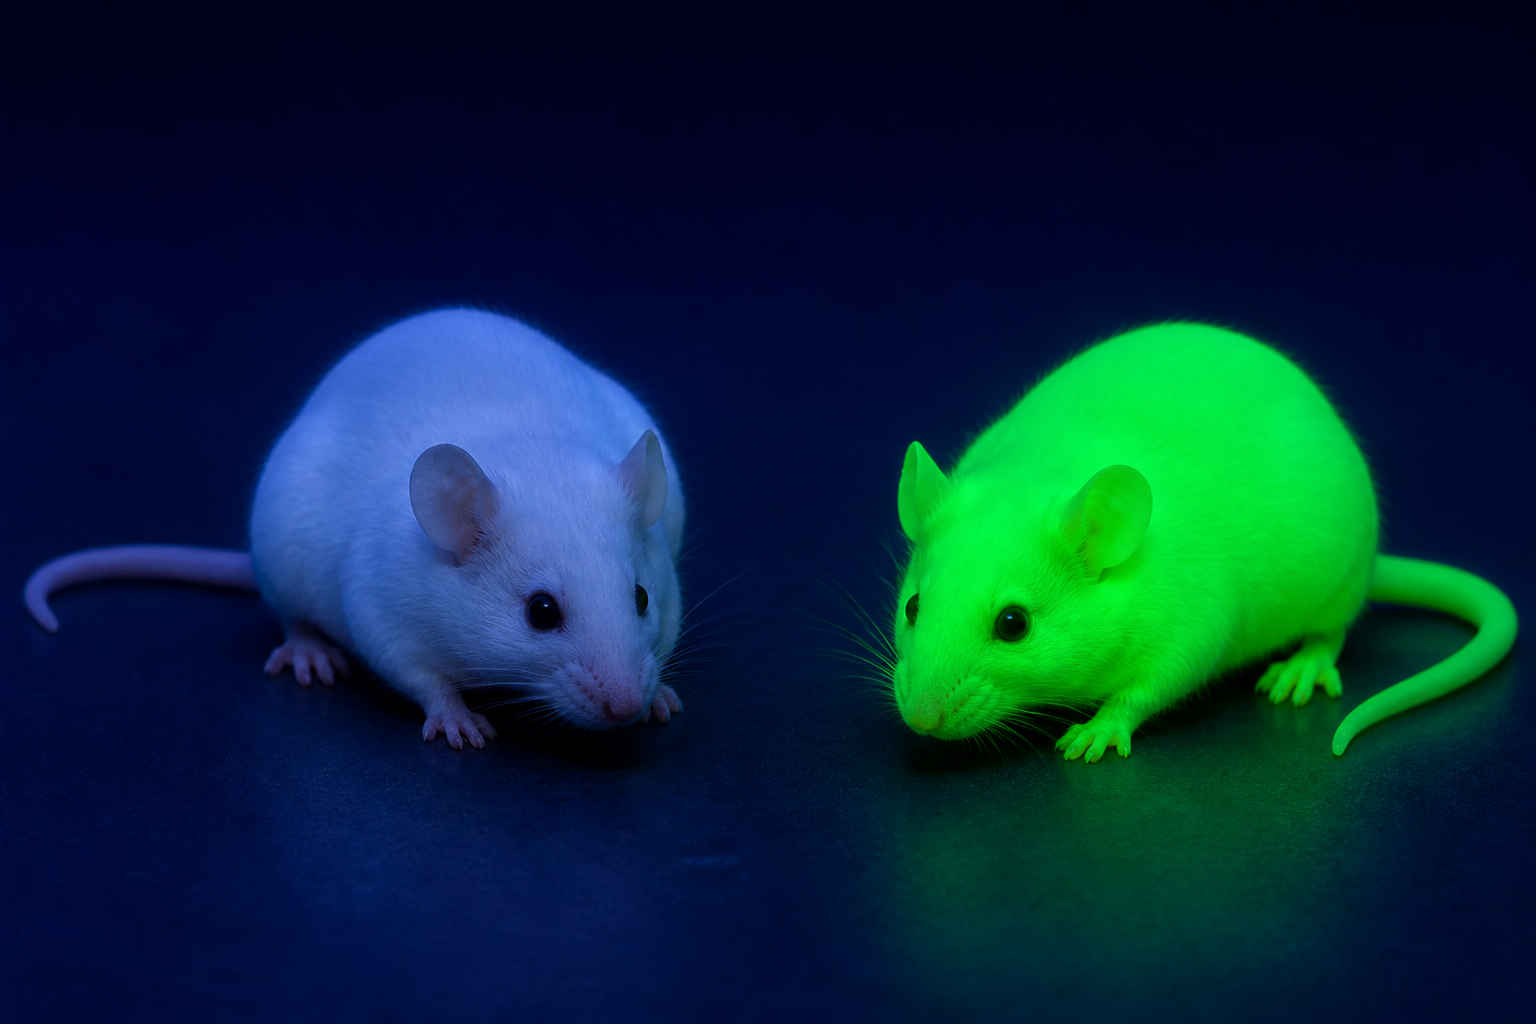
\includegraphics[width=0.62\linewidth]{images/book2/ai/g10-dna-gfp-mice.png}

{\small Bajo luz azul, un ratón que lleva el \omterm{def:g10:universal-dna:gene}{gen} de medusa de la
\omterm{def:g10:chemistry-of-life:families}{proteína} verde fluorescente brilla junto a un ratón corriente. Misma
molécula, mismas reglas de lectura: la instrucción de la medusa
funciona en el ratón.}
\end{omfigure}

\begin{example}[Usos de la transgénesis]\label{ex:g10:universal-dna:uses}
Insulina y hormona del crecimiento humanas obtenidas de bacterias; un
\omterm{def:g10:universal-dna:gene}{gen} de resistencia a un insecto plaga insertado en el maíz o en el
algodón; arroz con \omterm{def:g10:universal-dna:gene}{genes} para fabricar un precursor de la vitamina A;
el \omterm{def:g10:universal-dna:gene}{gen} de la GFP unido a otro \omterm{def:g10:universal-dna:gene}{gen} para que las \omterm{def:g10:cells-common-unit:cell}{células} en las que ese
\omterm{def:g10:universal-dna:gene}{gen} está activo se iluminen al microscopio --- este último uso, una
herramienta de investigación, es con diferencia el más frecuente. Cada
uso plantea sus propias preguntas de seguridad y de consecuencias para
el medio ambiente; todos descansan en el mismo hecho, la universalidad
de la molécula genética.
\end{example}

\begin{remark}[Unidad y diversidad en el plano molecular]\label{rem:g10:universal-dna:unity}
La universalidad del \omterm{def:g10:universal-dna:information}{ADN} es la cara molecular de la unidad de la vida
que aparece en el \cref{ch:g10:chemistry-of-life}: una química, una
molécula de información y un sistema de lectura para todos los
organismos de la Tierra, que es justo lo que predice un origen común
(\cref{ch:g10:common-ancestry}). La diversidad de la vida está escrita
también en la misma molécula, como diferencias de secuencia: entre dos
\omterm{def:g10:universal-dna:gene}{alelos}, unas pocas \omterm{def:g10:universal-dna:nucleotide}{bases}; entre dos especies, un pequeño porcentaje del
genoma; entre una bacteria y un humano, toda la organización del texto.
\end{remark}

\section{Ejercicios}

\begin{exercise}[$\star$]\label{exo:g10:universal-dna:1}
Nombra las tres partes de un \omterm{def:g10:universal-dna:nucleotide}{nucleótido} y las cuatro \omterm{def:g10:universal-dna:nucleotide}{bases} del \omterm{def:g10:universal-dna:information}{ADN}.
\end{exercise}

\begin{exercise}[$\star$]\label{exo:g10:universal-dna:2}
Escribe la hebra complementaria de \texttt{TACGGATTCA}.
\end{exercise}

\begin{exercise}[$\star$]\label{exo:g10:universal-dna:3}
Una muestra de \omterm{def:g10:universal-dna:information}{ADN} contiene un 21\% de guanina. Da los porcentajes de
C, de A y de T.
\end{exercise}

\begin{exercise}[$\star$]\label{exo:g10:universal-dna:4}
Define \omterm{def:g10:universal-dna:gene}{gen} y \omterm{def:g10:universal-dna:gene}{alelo} en una frase cada uno, usando la palabra
``secuencia''.
\end{exercise}

\begin{exercise}[$\star$]\label{exo:g10:universal-dna:5}
¿Qué es un organismo transgénico? Da dos ejemplos del capítulo.
\end{exercise}

\begin{exercise}[$\star\star$]\label{exo:g10:universal-dna:6}
Un \omterm{def:g10:universal-dna:gene}{gen} mide 1500 pares de \omterm{def:g10:universal-dna:nucleotide}{bases}. ¿Cuál es su longitud en nanómetros y
cuántas vueltas de hélice da?
\end{exercise}

\begin{exercise}[$\star\star$]\label{exo:g10:universal-dna:7}
Calcula la longitud total del \omterm{def:g10:universal-dna:information}{ADN} de una \omterm{def:g10:cells-common-unit:cell}{célula} humana, sabiendo que
hay $\num{3.2e9}$ pares de \omterm{def:g10:universal-dna:nucleotide}{bases} por juego de \omterm{def:g10:universal-dna:information}{cromosomas} y dos juegos
por \omterm{def:g10:cells-common-unit:cell}{célula}. Compárala con el diámetro del \omterm{def:g10:cells-common-unit:organelle}{núcleo}, \qty{6}{\micro m}.
\end{exercise}

\begin{exercise}[$\star\star$]\label{exo:g10:universal-dna:8}
En el experimento de Avery, ¿por qué hacía falta probar el extracto
tratado con una enzima destructora del \omterm{def:g10:universal-dna:information}{ADN}, y no solo la fracción de
\omterm{def:g10:universal-dna:information}{ADN} purificado?
\end{exercise}

\begin{exercise}[$\star\star$]\label{exo:g10:universal-dna:9}
Explica por qué los datos de Chargaff descartaban un modelo en el que
las \omterm{def:g10:universal-dna:nucleotide}{bases} se apilaran en un orden repetitivo regular como
\texttt{ATGCATGC\dots}
\end{exercise}

\begin{exercise}[$\star\star$]\label{exo:g10:universal-dna:10}
Dos \omterm{def:g10:universal-dna:gene}{alelos} de un \omterm{def:g10:universal-dna:gene}{gen} se diferencian en una sola base de entre 2000.
Explica cómo una diferencia tan pequeña puede cambiar una \omterm{def:g10:chemistry-of-life:families}{proteína}, y
por qué también puede no cambiar nada.
\end{exercise}

\begin{exercise}[$\star\star$]\label{exo:g10:universal-dna:11}
El \omterm{def:g10:universal-dna:gene}{gen} de la GFP insertado en el óvulo fecundado de un ratón se
encuentra en sus \omterm{def:g10:cells-common-unit:cell}{células} de la piel, en las del hígado y en sus
espermatozoides. Explica por qué, con la teoría celular y la
\cref{prop:g10:universal-dna:explains}.
\end{exercise}

\begin{exercise}[$\star\star\star$]\label{exo:g10:universal-dna:12}
La molécula de \omterm{def:g10:universal-dna:information}{ADN} de una bacteria mide $\num{4.6e6}$ pares de \omterm{def:g10:universal-dna:nucleotide}{bases}.
Calcula su longitud; compárala con los \qty{2}{\micro m} de la \omterm{def:g10:cells-common-unit:cell}{célula};
después explica por qué, aun así, una bacteria tiene sitio para ella.
\end{exercise}

\begin{exercise}[$\star\star\star$]\label{exo:g10:universal-dna:13}
Un amigo afirma que el \omterm{def:g10:universal-dna:information}{ADN} humano tiene que ser ``más complejo'' que el
de una bacteria porque tiene más \omterm{def:g10:universal-dna:nucleotide}{bases}. Compara $\num{3.2e9}$ y
$\num{4.6e6}$ pares de \omterm{def:g10:universal-dna:nucleotide}{bases} con $\num{20000}$ y 4300 \omterm{def:g10:universal-dna:gene}{genes}, y discute
qué es y qué no es ese \omterm{def:g10:universal-dna:information}{ADN} de más.
\end{exercise}

\begin{exercise}[$\star\star\star$]\label{exo:g10:universal-dna:14}
Supón que se descubriera una especie cuyo material genético usara otra
molécula y otro código. ¿Qué proposiciones del capítulo contradiría, y
qué implicaría sobre el origen común de esa especie y del resto de la
vida?
\end{exercise}

\begin{exercise}[$\star\star\star$]\label{exo:g10:universal-dna:15}
La insulina humana producida por bacterias sustituyó a la insulina
extraída de páncreas de cerdo. Enumera dos razones biológicas por las
que el producto bacteriano fue una mejora, y una pregunta que un
regulador aún tendría que plantear.
\end{exercise}

\section{Problema: El gen de la medusa}

\begin{problem}[{Problema de fin de semana --- un gen de medusa seguido
hasta un ratón: su longitud, sus letras, por qué el ratón puede leerlo
y los dos metros de ADN que lo llevan en cada célula}]
\label{pb:g10:universal-dna:1}
La \omterm{def:g10:chemistry-of-life:families}{proteína} verde fluorescente de la medusa \emph{Aequorea victoria} es
una cadena de 238 \omterm{def:g10:chemistry-of-life:families}{aminoácidos}. Su \omterm{def:g10:universal-dna:gene}{gen}, tal como se usa en el
laboratorio, es un segmento de \omterm{def:g10:universal-dna:information}{ADN} de 720 pares de \omterm{def:g10:universal-dna:nucleotide}{bases}. Toma
\qty{0.34}{nm} por par de \omterm{def:g10:universal-dna:nucleotide}{bases}, diez pares de \omterm{def:g10:universal-dna:nucleotide}{bases} por vuelta y un
genoma de ratón de $\num{2.7e9}$ pares de \omterm{def:g10:universal-dna:nucleotide}{bases} por juego de
\omterm{def:g10:universal-dna:information}{cromosomas}, con dos juegos por \omterm{def:g10:cells-common-unit:cell}{célula}.

\medskip
\noindent\textbf{Parte I --- La molécula.}
\begin{enumerate}
  \item Calcula la longitud del \omterm{def:g10:universal-dna:gene}{gen} de la GFP en nanómetros y el número
        de vueltas de hélice que da.
  \item Una hebra del \omterm{def:g10:universal-dna:gene}{gen} empieza por
        \texttt{ATGAGTAAAGGAGAAGAAC}. Escribe la hebra complementaria.
  \item En el \omterm{def:g10:universal-dna:gene}{gen} entero, la adenina representa el 27\% de las \omterm{def:g10:universal-dna:nucleotide}{bases}.
        Da los porcentajes de las otras tres \omterm{def:g10:universal-dna:nucleotide}{bases}.
  \item El \omterm{def:g10:universal-dna:gene}{gen} tiene 720 pares de \omterm{def:g10:universal-dna:nucleotide}{bases} y codifica 238 \omterm{def:g10:chemistry-of-life:families}{aminoácidos}.
        Calcula el cociente y propón qué sugiere sobre cuántas \omterm{def:g10:universal-dna:nucleotide}{bases}
        especifican un \omterm{def:g10:chemistry-of-life:families}{aminoácido} (una hipótesis que el
        \cref{ch:g11:gene-expression} confirmará).
  \item ¿Cuántas secuencias distintas de 720 \omterm{def:g10:universal-dna:nucleotide}{bases} son posibles en
        principio? Escribe la respuesta como una potencia de 4 y
        explica en una frase por qué la secuencia puede llamarse
        información.
\end{enumerate}

\medskip
\noindent\textbf{Parte II --- Por qué el ratón puede leerlo.}
\begin{enumerate}[resume]
  \item Enuncia la propiedad del \omterm{def:g10:universal-dna:information}{ADN} que permite a una \omterm{def:g10:cells-common-unit:cell}{célula} de ratón
        usar un \omterm{def:g10:universal-dna:gene}{gen} de medusa.
  \item El \omterm{def:g10:universal-dna:gene}{gen} se inserta en un óvulo fecundado y no en la piel de un
        ratón adulto. Con la teoría celular, explica qué diferencia
        supone esto respecto de dónde acaba el \omterm{def:g10:universal-dna:gene}{gen}.
  \item El ratón adulto brilla en todos sus tejidos. ¿Qué muestra esto
        sobre el contenido de \omterm{def:g10:universal-dna:information}{ADN} de sus distintos tipos celulares?
  \item El ratón que brilla se cruza con un ratón corriente. Predice,
        con una razón, si brillará parte de la descendencia.
  \item A un ratón de control se le inyecta \omterm{def:g10:chemistry-of-life:families}{proteína} GFP purificada en
        lugar del \omterm{def:g10:universal-dna:gene}{gen}: brilla débilmente unos días y luego deja de
        hacerlo. Explica la diferencia entre los dos experimentos.
\end{enumerate}

\medskip
\noindent\textbf{Parte III --- Las pruebas que hay detrás.}
\begin{enumerate}[resume]
  \item En el experimento de Avery, nombra la fracción que transformaba
        las bacterias y el tratamiento que suprimía la transformación.
  \item Explica por qué el experimento de transformación es una versión
        natural de la \omterm{prop:g10:universal-dna:universal}{transgénesis}.
  \item Chargaff encontró A$\,=\,$T y G$\,=\,$C en todas las especies,
        pero con A+T variando del 25\% al 75\%. ¿Cuál de las dos
        observaciones apoya el emparejamiento de \omterm{def:g10:universal-dna:nucleotide}{bases} y cuál muestra
        que la secuencia es libre?
  \item Las fotografías de Franklin dieron un diámetro de hélice de
        \qty{2}{nm}. Explica por qué emparejar una base grande con una
        pequeña (A con T, G con C) en lugar de dos grandes hace regular
        la hélice.
  \item ¿Por qué el descubrimiento de la estructura sugirió de
        inmediato cómo se copia el \omterm{def:g10:universal-dna:information}{ADN}?
\end{enumerate}

\medskip
\noindent\textbf{Parte IV --- Dos metros en un \omterm{def:g10:cells-common-unit:organelle}{núcleo}.}
\begin{enumerate}[resume]
  \item Calcula la longitud total del \omterm{def:g10:universal-dna:information}{ADN} de una \omterm{def:g10:cells-common-unit:cell}{célula} de ratón.
  \item El \omterm{def:g10:cells-common-unit:organelle}{núcleo} mide \qty{6}{\micro m} de lado a lado. ¿Por qué
        factor debe acortarse el \omterm{def:g10:universal-dna:information}{ADN} al plegarse para caber?
  \item ¿Qué fracción del \omterm{def:g10:universal-dna:information}{ADN} de la \omterm{def:g10:cells-common-unit:cell}{célula} es el \omterm{def:g10:universal-dna:gene}{gen} de la GFP?
  \item Un ratón tiene unos $\num{2e4}$ \omterm{def:g10:universal-dna:gene}{genes} de $\num{3e4}$ pares de
        \omterm{def:g10:universal-dna:nucleotide}{bases} de media, contando sus partes no codificantes. ¿Qué
        fracción del genoma ocupan los \omterm{def:g10:universal-dna:gene}{genes}?
  \item Enuncia el resultado en una frase: ¿cuánto \omterm{def:g10:universal-dna:information}{ADN} lleva una \omterm{def:g10:cells-common-unit:cell}{célula}
        de ratón y qué único hecho sobre ese \omterm{def:g10:universal-dna:information}{ADN} permite leer un \omterm{def:g10:universal-dna:gene}{gen} de
        medusa entre sus miles de \omterm{def:g10:universal-dna:gene}{genes}?
\end{enumerate}
\end{problem}
